\chapter{Indexing}
\index{Indexing|(}

Trees tend to put on big rings when they're young, and smaller rings when they get older. Some trees put on very large rings, while others put on very small rings. These variations in growth can make it difficult to crossdate samples.  Some dendrochronologists therefore prefer to index or normalize their ring width data before combining into chronologies.

Indexing is a manipulation you can perform on your data to make it easier to crossdate.

The procedure for indexing is as follows:

\begin{enumerate*}
   \item You open a series (raw data)
   \item You ask Corina to index it
   \item Corina shows you some possible curves
   \item You pick a curve (based on its graph, statistical scores, and your expectation of how the tree is growing)
   \item Corina converts each year's ring width to a ratio of actual growth to expected growth for that year
   \item You save the series (indexed data) 
\end{enumerate*}

Indexing changes the units of a dataset. A raw sample has units of hundredths of a millimeter (0.01 mm) or microns. An indexed sample has units of parts per thousand (0.1\%, or \textperthousand).

This doesn't cause a problem with crossdating. The t-score normalizes all samples as part of its test, and the trend only cares if the values are increasing or decreasing. For more information on crossdating and chronology building, see chapter \ref{txt:crossdating}.  It does, however, cause a problem with `summing' since summing needs to take the average (what's the average of 1mm and 75\%?). Therefore, the samples in a sum must be either all raw, or all indexed. 

\section{Types of index}

There are a total of six different indexing methods available in Corina:

\subsection{Exponential Index}
\index{Indexing!Exponential}
\index{Expontential index|see{Indexing}}
This is the most commonly used index as it matches the way trees typically grow. Quickly when young and then gradually slower.  An exponential index is therefore by far the most common index you'll use as 9 times out of 10 this will be the best choice. 

This index tries to fit an equation of the following form to your data, searching for the best values of $a$, $b$ and $p$. 
\begin{itemize}
 \item $y = a + be-px$ 
\end{itemize}

\info{This is sometimes called a negative exponential index, because the exponent is negative. Corina doesn't require that the exponent is negative, but if it's not, using this index probably isn't such a good idea; it means the tree is generally getting bigger, not smaller.}

The least-squares algorithm used comes from \citet{CLR}; the matrix solving function comes from \citet{vanLoan}.

Sometimes the exponential index does a lousy job. If a tree is living in a crowded area and the trees around it get cut down, suddenly it has much better growing conditions, so it might grow faster as it gets older, instead of slower. If you tried to use an exponential curve on a tree like this, it would exaggerate this growth, and useful data would get flattened out.

The result is you're looking at the growing conditions of this one tree, so it's not going to crossdate as well.

Alternatively, imagine you are working on a tree with a fire scar that has a few very large rings. An exponential index wouldn't take much notice of this, because most of the sample is still shaped like an exponential curve, but when you applied it they would be grossly out of proportion. For these types of samples, there are other indexing algorithms available.


\subsection{Polynomial Index}
\index{Indexing!Polynomial}
\index{Polynomial index|see{Indexing}}
When you ask Corina to perform a Polynomical Index it tries to fit a polynomial curve to your data using the following equation: 

\begin{itemize}
\item $y = a_{n}x^{n} + a_{n-1}x^{n-1} + \dots + a_{2}x^{2} + a_{1x} + a_{0}$ 
\end{itemize}

You decide what degree polynomial, n, to use and Corina automatically finds the best values of $a_{0}$, $a_{1} \dots a_{n}$, to fit your data. 

\subsection{Horizontal Line Index}
\index{Indexing!Horizontal}
\index{Horizontal index|see{Indexing}}
This only changes the magnitude not shape of the curve and is used when you would link to combine raw and indexed data together.  It is a special case of polynomial where the horizontal line is equal to the average value. 

\begin{itemize}
\item $y = x_{avg}$
\end{itemize}

This index is not used for crossdataing because dividing each value by the same value doesn't change the shape of the curve, only its magnitude. A horizontal line index is, however, useful because every element in a sum must use the same units, either raw or indexed. Therefore if you want to include a raw sample with an indexed sample then a horizontal line index can be used to convert the raw sample without otherwise altering the shape of the curve. 

\subsection{Floating Index}
\index{Indexing!Floating}
\index{Floating index|see{Indexing}}
This is a running average of the 11 surrounding years. The adaptive index is generally used as a `last resort' when both exponential and a high-degree polynomial have failed. It is simply the average of the eleven surrounding years:

\begin{itemize}
\item $ind_{i} = 1/11 (data-{i-5} + data_{i-4} + \dots + data_{i+4} + data_{i+5})$ 
\end{itemize}

This index was originally called floating average, probably in reference to the fact that the index curve ``floats'' around, not following any explicit $y=f(x)$-type formula. But people tended to call it floating, and then floating-point, which means something very different. You might still hear people calling this index by these other names.

\subsection{High-Pass Filter Index}
\index{Indexing!High-pass filter}
\index{High-pass filter|see{Indexing}}
The high-pass index is a more general case of the adaptive index. Instead of simply taking the average of 11 values, it takes a weighted average. It's an example of a ``high-pass'' filter because high-frequency signals can pass through, but low-frequency signals are filtered out.

The default is ``1-2-4-2-1'', meaning:

\begin{itemize}
\item $ind_{i} = 1/10 (data_{i-2} + 2{\cdotp}data_{i-1} + 4{\cdotp}data_{i} +2{\cdotp}data_{i+1} + data_{i+2})$ 
\end{itemize}

This comes from \citet{Cook81} who used it as a discrete filter before moving to a cubic spline. Note that almost half ($4/10$) of the computed value is simply its old value. The high-pass index is nearly the same as the input, so the $\chi^2$ values are usually the lowest, therefore do not choose this index solely on a low $\chi^2$ value. 

\subsection{Cubic Spline Index}
\index{Indexing!Cublic spline}
\index{Cublic spline|see{Indexing}}
Cubic splines are a very specific type of high-pass filter. A cubic spline curve is created by combining a collection of cubic (3rd degree polynomial) functions.

There are many methods for constructing cubic splines through a dataset. The algorithm used by Corina has a parameter, s, which controls how tightly the spline fits the data. A lower value fits the data more tightly, a higher value fits the data more loosely. Therefore, s=0 fits the data exactly while s=1 is a simple line. A good starting point for dendro data seems to be around $s=1x1016$.

Cubic splines were first used for dendro by \citet{Cook81} using an algorithm from \citet{Reinsch67}.

You can change the s-value used for the subic spline in the preferences. You might use a cubic spline in the same cases you would use a high-pass filter e.g.\ when the sample doesn't generally follow an exponential or polynomial curve very well, perhaps due to a fire scar. 

\section{Indexing data}
\index{Indexing|textbf}
To index your data, first you need to open the series you would like to index.  Next choose \menutwo{Tools}{Index} to display the indexing dialog (figure \ref{fig:index}).

\begin{figure}[hbtp]
  \centering
    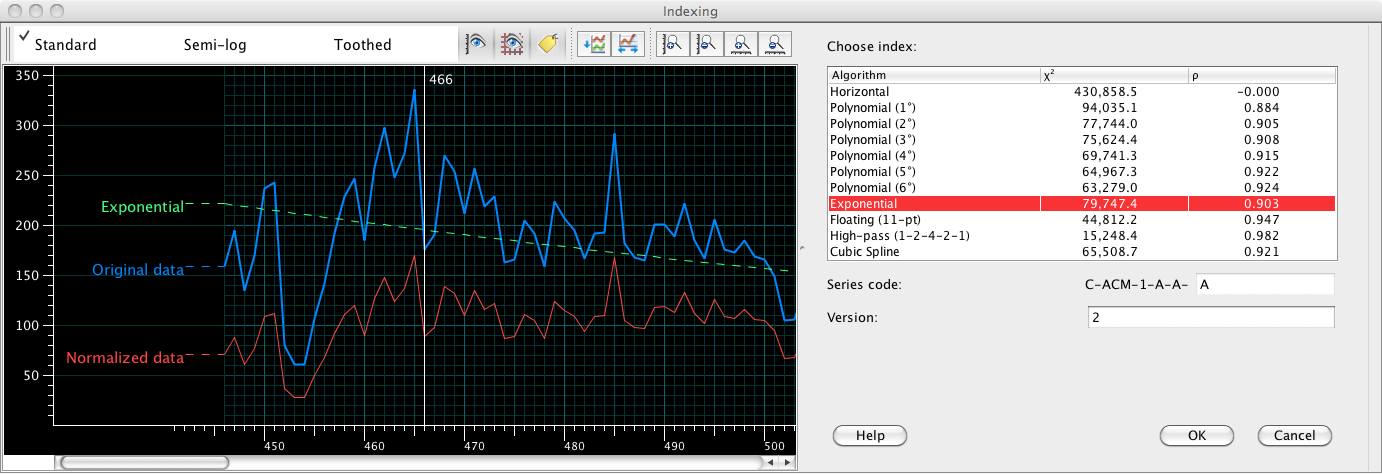
\includegraphics[width=0.97\textwidth]{Images/index.png}
    \caption{Indexing dialog showing the original data in blue, the exponential index of this data in green, and the normalized data in red. }
    \label{fig:index}
\end{figure}

From the indexing dialog you can then choose which type of index to apply to your data.  The table on the right shows the available options along with the $\chi^2$ and p values to help you choose the correct index to use. The graph shows your original data, the index line and the result of applying the index to the data and changes dynamically as you pick between different indexing methods. Once you have decided which index you want to use, select it, and click OK ensuring that you have given your data series a new version number.

\index{Indexing|)}